% !TEX spellcheck = en_US



% ~~~~~~~~~~~~~~~~~~~~~~~~~~~~~~~~~~~~~~~ V
% (NC) 2024Haluk Bingol
% github.com/halukbingol/LaTeX-Templates
%
% Licensees may copy, distribute, display, and perform the work and make derivative works 
% and remixes based on it only for non-commercial purposes. 
% ~~~~~~~~~~~~~~~~~~~~~~~~~~~~~~~~~~~~~~~ A




%\documentclass{beamer}
\documentclass[10pt]{beamer}
	\usetheme{Dresden}
%	\usetheme{Copenhagen}
%	\usetheme{Marburg}
%	\usetheme{CambridgeUS}
%	\usetheme{Warsaw}
%	\usetheme{AnnArbor}

%	\usecolortheme{orchid}
	
%	\usecolortheme{}
%	\useinnertheme{}
%	\useoutertheme{}
%	\setbeamertemplate{bibliography item}[text]
\usepackage{beamerthemesplit}
%\usecolortheme{default}
%\usecolortheme{structure}
%\usepackage{beamerthemesplit} // Activate for custom appearance

\useoutertheme{split}
\usecolortheme{whale}
\useinnertheme{rounded} 
\usecolortheme{orchid}
\setbeamertemplate{blocks}[rounded]




% ~~~~~~~~~~~~~~~~~~~~~~~~~~~~~~~~~~~~~~~ V HB lib
\usepackage{../hbcommon/hbdatastructures} 
\usepackage{../hbcommon/hbpresentation} 
% ~~~~~~~~~~~~~~~~~~~~~~~~~~~~~~~~~~~~~~~ A




% ~~~~~~~~~~~~~~~~~~~~~~~~~~~~~~~~~~~~~~~ V specific	
\usepackage[normalem]{ulem} %strikethroug

\usepackage{tikz-qtree} % tree
\usepackage{adjustbox} % tikzpicture alignment

%\usepackage{moreverb} % tab control
\usepackage{fancyvrb} % tab

\usepackage{epstopdf} % eps 2 pdf
\epstopdfsetup{update} % only regenerate pdf files when eps file is newer


\newcommand{\hDummy}{dummy}

% beamer blocks
% https://tex.stackexchange.com/questions/347269/different-colors-for-different-types-of-blocks-in-beamer
% https://tex.stackexchange.com/questions/28760/custom-beamer-blocks-for-pros-and-cons/

% https://tex.stackexchange.com/questions/1858/stable-vertical-alignment-of-columns-in-beamer
% https://tex.stackexchange.com/questions/127027/vertical-alignment-of-tikz-picture-in-a-table-cell
% https://tex.stackexchange.com/questions/172434/drawing-vertical-hierarchical-n-ary-tree-in-tikz
%  ~~~~~~~~~~~~~~~~~~~~~~~~~~~~~~~~~~~~~~~ A




% ~~~~~~~~~~~~~~~~~~~~~~~~~~~~~~~~~~~~~~~ V
%	\newcommand{\hAbs}[1]{\ensuremath{\left \lvert \, #1 \, \right \rvert} } % |x|
%	\newcommand{\hMean}[1]{\ensuremath{<\!\! #1 \!\!>}} % average
%	\newcommand{\hMean}[1]{\ensuremath{\overline{#1}}}
% ~~~~~~~~~~~~~~~~~~~~~~~~~~~~~~~~~~~~~~~ A


%: ==== HB Header Common Packages v20160423 ====V
	\usepackage[utf8]{inputenc} % To use Unicode characters
	\usepackage[iso]{datetime}
	%	\usepackage{etex}
	
%	\usepackage[a4paper]{geometry}
	
	\usepackage{xcolor}
	% black, blue, brown, cyan, darkgray, gray, green, lightgray, lime, 
	% magenta, olive, orange, pink, purple, red, teal, violet, white, yellow
%	\usepackage[colorlinks=true,linkcolor=red,urlcolor=blue,citecolor=red]%
%		{hyperref}
	\usepackage{graphicx,epstopdf}
	% \graphicspath{{fig}}
%	\graphicspath{{../common/figures/}}
	% \DeclareGraphicsExtensions{.pdf,.jpeg,.png,.eps}
	% \DeclareGraphicsRule{.tif}{png}{.png}%
	%	{`convert #1 `dirname #1`/`basename #1 .tif`.png}
%	\usepackage{subfigure}
%\usepackage{subfig}
%\usepackage{subcaption}
% ~~~~~~~~~~~~~~~~~~~~~~~~~~~~~~~~~~~~~~~ V HB Header Common Packages v20160423 




% ~~~~~~~~~~~~~~~~~~~~~~~~~~~~~~~~~~~~~~~ V
\title{
	cis112\\
	Binary Search Trees
}

\author[Bingol]{Haluk O. Bingol}

\institute{
	Faculty of Computer and Information Sciences\\
	Yeditepe University
}

%\date{
%	cis112\\ 
%	Yeditepe University, 2024-02-25
%}
\date{
	{\tiny v2026-05-03}
}
% ~~~~~~~~~~~~~~~~~~~~~~~~~~~~~~~~~~~~~~~ A



\begin{document}
% ~~~~~~~~~~~~~~~~~~~~~~~~~~~~~~~~~~~~~~~ 




% ~~~~~~~~~~~~~~~~~~~~~~~~~~~~~~~~~~~~~~~ V Title
\frame{\titlepage}
% ~~~~~~~~~~~~~~~~~~~~~~~~~~~~~~~~~~~~~~~ A 




% ~~~~~~~~~~~~~~~~~~~~~~~~~~~~~~~~~~~~~~~ V Content
\begin{frame}[t]\frametitle{Content}
	\begin{columns}[T]
	\begin{column}{.5\linewidth}
	    	\tableofcontents[hideallsubsections]
	\end{column}
	\begin{column}{.5\linewidth}
		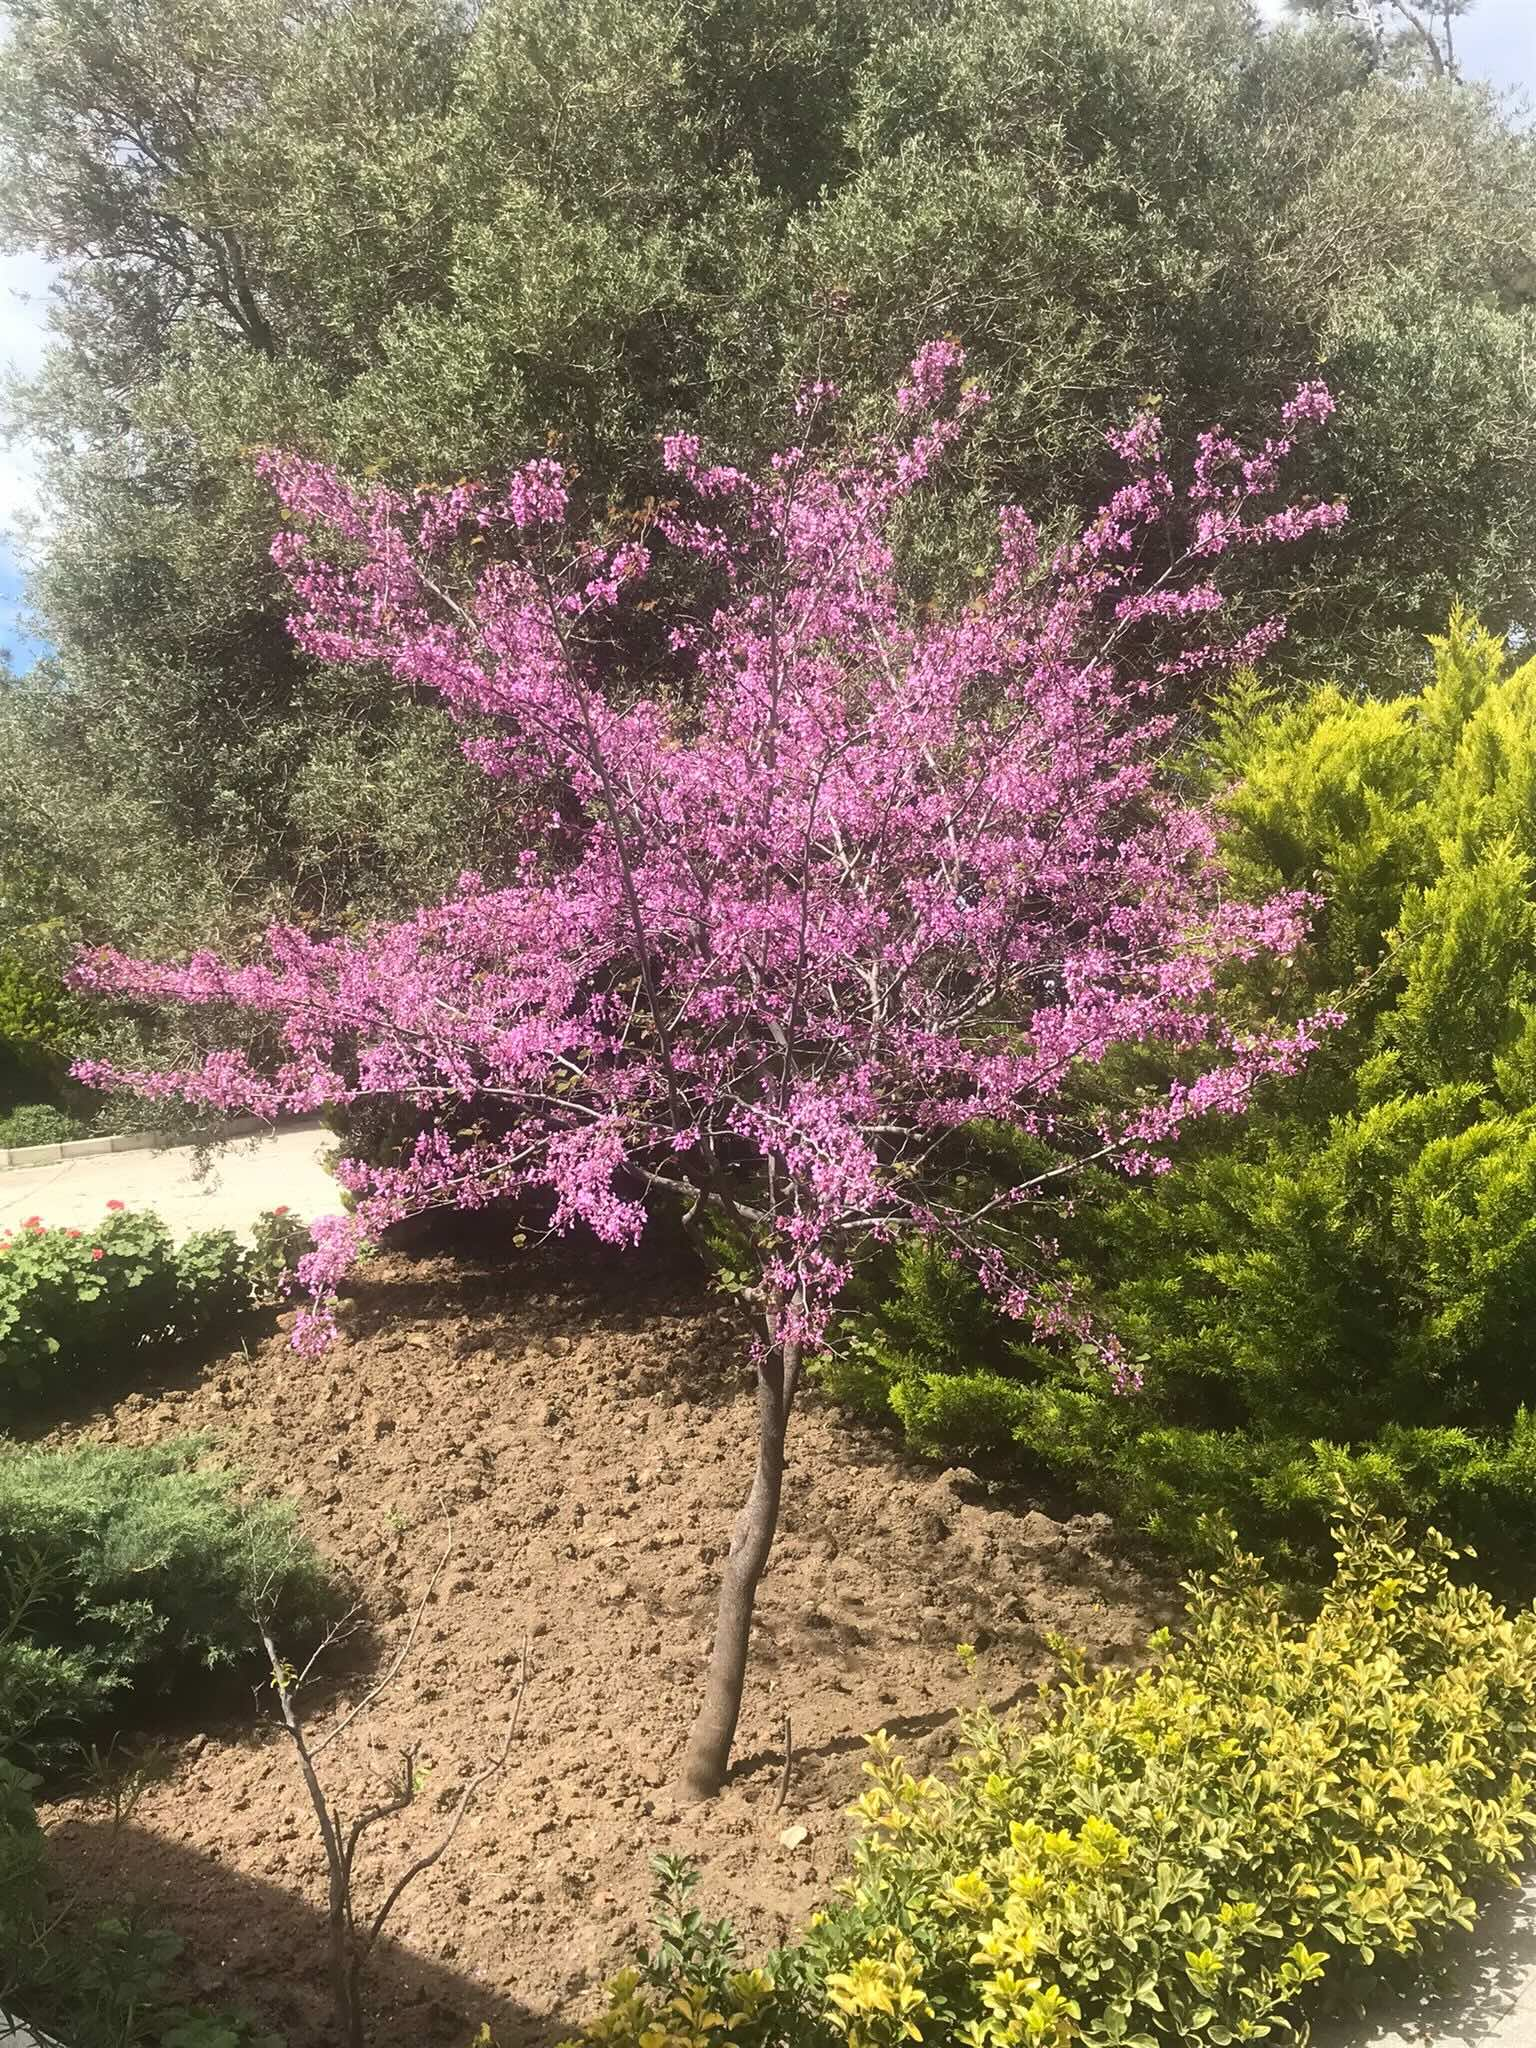
\includegraphics[width=.8\columnwidth]
		{fig/fig-Erguvan.jpg}
%		{example-image}
	\end{column}
	\end{columns}
\end{frame}
% ~~~~~~~~~~~~~~~~~~~~~~~~~~~~~~~~~~~~~~~ A




% ~~~~~~~~~~~~~~~~~~~~~~~~~~~~~~~~~~~~~~ V
\hSection{Motivation}{}{}
% ~~~~~~~~~~~~~~~~~~~~~~~~~~~~~~~~~~~~~~ A




\subsection{Finding hidden number}
% ~~~~~~~~~~~~~~~~~~~~~~~~~~~~~~~~~~~~~~ V
\begin{frame}[t,fragile] \frametitle{Game of secret number}
%\begin{frame}[t]\frametitle{aaa}
	\begin{columns}[T] % >>>>
	\begin{column}{.6\linewidth} % ++++ V
	
		\textbf{Game.}
		\begin{itemize}
			
			\item 
			Player-A selects a secret number in the range of \( \{ 1, 2, \dotsc, 8 \} \).
	
			\item
			Game repeats till the secret is found.
			
			\begin{itemize}
		
				\item 
				Player-B tries a number.
				
				\item 
				Player-A should answer as``found'', or ``smaller'' or ``larger''.
				
			\end{itemize}		
			
		\end{itemize}
	
		\textbf{Q.}
		What is the best strategy if the range becomes large 
		such as \( \{ 1, 2, \dotsc, 1000,000 \} \).
		
	\end{column} % ++++ A
	\begin{column}{.25\linewidth} % ++++ V
		\begin{tikzpicture}
			\tikzset{every leaf node/.style={font=\sffamily}}
			\Tree
			[.{4}
				[.$2$
					[.$1$ ]
					[.$3$ ]
				]
				[.$6$
					[.$5$  ]
					[.$7$  ]
				]
			]
		\end{tikzpicture}
		
		This strategy finds the secret faster.
	\end{column} % ++++ A
	\begin{column}{.15\linewidth} % ++++ V
		\begin{tikzpicture}
			\tikzset{every leaf node/.style={font=\sffamily}}
			\Tree
			[.$4$
				[.$3$
					[.$2$ 
					[.$1$ ]
					]
				]
				[.$5$
					[.$6$ 
						[.$7$ 
							[.$8$ ]
						]
					]
				]
			]
		\end{tikzpicture}
		
		This strategy is slower.
	\end{column} % ++++ A
	\end{columns} % <<<<
\end{frame}
% ~~~~~~~~~~~~~~~~~~~~~~~~~~~~~~~~~~~~~~ A




% ~~~~~~~~~~~~~~~~~~~~~~~~~~~~~~~~~~~~~~ V
\hSection{Definitions}{}{}
% ~~~~~~~~~~~~~~~~~~~~~~~~~~~~~~~~~~~~~~ A




% ~~~~~~~~~~~~~~~~~~~~~~~~~~~~~~~~~~~~~~ V
\begin{frame}[t]\frametitle{Binary Search Tree}
	\begin{columns}[T] % >>>>
	\begin{column}{.55\linewidth} % ++++ V
		{\footnotesize 
			\begin{definition}
				\hDefined{Binary search tree property} :
				
				Let $x$ be a node in a binary tree.
				
				\begin{enumerate}
				
					\item 
					If $y$ is a node in the \hEmph{left subtree} of $x$,
					then $y.data \le x.data$.
				
					\item 
					If $y$ is a node in the \hEmph{right subtree} of $x$,
					then $y.data \ge x.data$.
				\end{enumerate}
						
				A binary tree with the binary-search-tree property 
				is called a \hDefined{binary search tree}.\\
			\end{definition}
		} %fsize
				
		\vspace{1cm}
		\hCite{ %
	\cite{knuth1973artv1}, %
	\cite{cormen2022introduction}, %
	\cite{preiss1999}, %
	\cite{aho1974design}, %
	\cite{horowitz1982fundamentals}, %
	\cite{horstmann2016big}, %
	\cite{grimaldi2006discrete}
}

	\end{column} % ++++ A
	\begin{column}{.45\linewidth} % ++++ V
		\begin{example}
		{\scriptsize
			\begin{tikzpicture}
	\tikzset{every leaf node/.style={font=\sffamily}}
	\Tree
	[.$6$
		[.$5$
			[.$2$ ]
			[.$5$ ]
		]
		[.$7$
			[. ~ ]
			[.$8$ ]
		]
	]
\end{tikzpicture}

			\\		
			2 is in the left subtree of 5 since $2 \le 5$.\\
			2 is in the left subtree of 6 since $2 \le 6$.\\
			8 is in the right subtree of 7 since $8 \ge 7$.\\
			8 is in the right subtree of 6 since $8 \ge 6$.\\
			\hCite{
				\cite{cormen2022introduction}
			}

		} %\scriptsize
		\end{example}

	\end{column} % ++++ A
	\end{columns} % <<<<
\end{frame}
% ~~~~~~~~~~~~~~~~~~~~~~~~~~~~~~~~~~~~~~ A




% ~~~~~~~~~~~~~~~~~~~~~~~~~~~~~~~~~~~~~~ V
\hSection{Algorithms}{}{}
% ~~~~~~~~~~~~~~~~~~~~~~~~~~~~~~~~~~~~~~ A




%% ~~~~~~~~~~~~~~~~~~~~~~~~~~~~~~~~~~~~~~ V
%\hSubsection{Algorithms}{Node}
%% ~~~~~~~~~~~~~~~~~~~~~~~~~~~~~~~~~~~~~~ A



% ~~~~~~~~~~~~~~~~~~~~~~~~~~~~~~~~~~~~~~ V
\begin{frame}[t]\frametitle{Node}
	\begin{columns}[T] % >>>>
	\begin{column}{.6\linewidth} % ++++ V
		{\tiny 
			\begin{algorithm}[H]
	\SetKwData{Data}{\texttt{data}}
	\SetKwData{P}{\texttt{parent}}
	\SetKwData{L}{\texttt{left}}
	\SetKwData{R}{\texttt{right}}
	\Begin{
		\Data\\
		\P	\tcp*[f]{{\tiny reference to the parent}}\\
		\L	\tcp*[f]{{\tiny reference to the left child}}\\
		\R	\tcp*[f]{{\tiny reference to the right child}}\\
	    
		\caption{{\footnotesize Node for Binary Search Tree}}
	}
\end{algorithm}

\hCite{%
	\cite{cormen2022introduction}%
}
		} % fsize
		
		{\footnotesize 
		\textbf{Warning.}
		\texttt{data} is comparable:\\
		Comparison of  \hCode{a.data} and \hCode{b.data} 
		for \texttt{Node}s,  \hCode{a} and \hCode{b}, is defined as
		\[
			\hCode{a.data.comparedTo(b.data)} = 
			\begin{cases}
				< 0, & \hCode{a.data < b.data}, \\
				0, & \hCode{a.data == b.data},\\
				> 0, & \hCode{a.data > b.data}.
			\end{cases}
		\]
		} % fsize		
	\end{column} % ++++ A
	\begin{column}{.4\linewidth} % ++++ V
		{\footnotesize 
%		\begin{tikzpicture}
	\tikzset{every leaf node/.style={font=\sffamily}}
	\Tree
	[.{parent} 
		[.l  \edge[roof]; {leftSubtree} ]
		[.r \edge[roof]; {rightSubtree} ]
	]
\end{tikzpicture}

		\begin{tikzpicture}
	\tikzset{every leaf node/.style={font=\sffamily}}
	\Tree
	[.\hEmph{parent}
		[.\hEmph{node} 
			[.\hEmph{$root_{T_{L}}$}   \edge[roof]; {subtree-$T_{L}$} ]
			[.\hEmph{$root_{T_{R}}$}   \edge[roof]; {subtree-$T_{R}$} ]
		]
	]
\end{tikzpicture}		

		} % fsize
	\end{column} % ++++ A
	\end{columns} % <<<<
	
\end{frame}
% ~~~~~~~~~~~~~~~~~~~~~~~~~~~~~~~~~~~~~~ A




% ~~~~~~~~~~~~~~~~~~~~~~~~~~~~~~~~~~~~~~ V
\hSubsection{Algorithms}{Tree Traversal}
% ~~~~~~~~~~~~~~~~~~~~~~~~~~~~~~~~~~~~~~ A




% ~~~~~~~~~~~~~~~~~~~~~~~~~~~~~~~~~~~~~~ V
\begin{frame}[t]\frametitle{Inorder Tree Traversal}
	\begin{columns}[T] % >>>>
	\begin{column}{.6\linewidth} % ++++ V
{\footnotesize 
		\begin{function}[H]
	\SetKwData{X}{\texttt{x}}
	\SetKwData{Left}{\texttt{left}}
	\SetKwData{Right}{\texttt{right}}
	\SetKwData{Data}{\texttt{data}}
	\SetKwData{N}{\texttt{NIL}}

%	\FuncSty{InorderTreeWalk(}\ArgSty{\X}\FuncSty{)}\\
		\If{\X $\neq$ NIL}{
			InorderTreeWalk(\X.\Left)\\
			print \X.\Data\\
			InorderTreeWalk(\X.\Right)\\
		}
	\caption{InorderTreeWalk(x)
		\hCite{%
			\cite{cormen2022introduction}%
		}	
	}
\end{function}

} % fsize

	\end{column} % ++++ A
	\begin{column}{.4\linewidth} % ++++ V

		{\small 
		\begin{tikzpicture}
	\tikzset{every leaf node/.style={font=\sffamily}}
	\Tree
	[.$15$
		[.$6$
			[.$3$ 
				[.$2$ ]
				[.$4$ ]
			]
			[.$7$
				[.$~$ ]
				[.$13$ 
					[.$9$ ]
					[.$~$ ]
				]				
			]
		]
		[.$18$
			[.$17$ ]
			[.$20$ ]
		]
	]
\end{tikzpicture}

		} % fsize


		{\footnotesize 
			\begin{tabular}{| l |}
			\hline
			Output of {\scriptsize \InorderTreeWalk(15)}\\
			\hline
			2, 3, 4, 6, 7, 9, 13, 15, 17, 18, 20.\\
			\hline
			\end{tabular}
		} % fsize

	\end{column} % ++++ A
	\end{columns} % <<<<
	
\end{frame}
% ~~~~~~~~~~~~~~~~~~~~~~~~~~~~~~~~~~~~~~ A




% ~~~~~~~~~~~~~~~~~~~~~~~~~~~~~~~~~~~~~~ V
\hSubsection{Algorithms}{Searching}
% ~~~~~~~~~~~~~~~~~~~~~~~~~~~~~~~~~~~~~~ A




% ~~~~~~~~~~~~~~~~~~~~~~~~~~~~~~~~~~~~~~ V
\begin{frame}[t]\frametitle{Tree Search}
	\begin{columns}[T] % >>>>
	\begin{column}{.6\linewidth} % ++++ V
	
		{\footnotesize
				\begin{function}[H]
	\SetKwData{X}{\texttt{x}}
	\SetKwData{K}{\texttt{k}}
	\SetKwData{N}{\texttt{NIL}}
	%
	\SetKwData{Left}{\texttt{left}}
	\SetKwData{Right}{\texttt{right}}
	\SetKwData{Data}{\texttt{data}}
	\SetKwData{Key}{\texttt{key}}

%	\FuncSty{TreeSearch(}\ArgSty{\X, \K}\FuncSty{)}\\
		\If {\X == \N or \Key == \X.\Key}{
			\Return \X
		}
		\If { \K $<$ \X.\Key }{
			\Return TreeSearch( \X.\Left, \K )
		} \Else {
			\Return TreeSearch( \X.\Right, \K )
		}
	\caption{TreeSearch(x, k)
		\hCite{%
			\cite{cormen2022introduction}%
		}	
	}
\end{function}

		} % fsize

		\vspace{1cm}
		{\footnotesize 
			\begin{tabular}{| l |}
			\hline
			Trace of {\scriptsize \TreeSearch(15, 14)}\\
			\hline
			\TreeSearch(15,14)\\
			\TreeSearch(6,14)\\
			\TreeSearch(7,14)\\
			\TreeSearch(13,14)\\
			\TreeSearch(NIL,14)\\
			\hline
			\end{tabular}
		} % fsize

	\end{column} % ++++ A
	\begin{column}{.4\linewidth} % ++++ V

		{\small 
		\begin{tikzpicture}
	\tikzset{every leaf node/.style={font=\sffamily}}
	\Tree
	[.$15$
		[.$6$
			[.$3$ 
				[.$2$ ]
				[.$4$ ]
			]
			[.$7$
				[.$~$ ]
				[.$13$ 
					[.$9$ ]
					[.$~$ ]
				]				
			]
		]
		[.$18$
			[.$17$ ]
			[.$20$ ]
		]
	]
\end{tikzpicture}

		} % fsize

		{\footnotesize 
			\begin{tabular}{| l |}
			\hline
			Trace of {\scriptsize \TreeSearch(15, 13)}\\
			\hline
			\TreeSearch(15,13)\\
			\TreeSearch(6,13)\\
			\TreeSearch(7,13)\\
			\TreeSearch(13,13)\\
			\hline
			\end{tabular}
		} % fsize

	\end{column} % ++++ A
	\end{columns} % <<<<
	
\end{frame}
% ~~~~~~~~~~~~~~~~~~~~~~~~~~~~~~~~~~~~~~ A




% ~~~~~~~~~~~~~~~~~~~~~~~~~~~~~~~~~~~~~~ V
\begin{frame}[t]\frametitle{Iterative Tree Search}
	\begin{columns}[T] % >>>>
	\begin{column}{.6\linewidth} % ++++ V
{\footnotesize
		\begin{function}[H]
	\SetKwData{X}{\texttt{x}}
	\SetKwData{K}{\texttt{k}}
	\SetKwData{N}{\texttt{NIL}}
	%
	\SetKwData{Left}{\texttt{left}}
	\SetKwData{Right}{\texttt{right}}
	\SetKwData{Data}{\texttt{data}}
	\SetKwData{Key}{\texttt{key}}

%	\FuncSty{IterativeTreeSearch(}\ArgSty{\X, \K}\FuncSty{)}\\
		\While {\X $\neq$ \N and \K $\neq$ \X.\Key}{
			\If {\K $<$ \X.\Key}{
				\X = \X.\Left
			}\Else {
				\X = \X.\Right	
			}
		}
		\Return \X
	
	\caption{IterativeTreeSearch(x, k)
		\hCite{%
			\cite{cormen2022introduction}%
		}	
	}
\end{function}

} % fsize

	\end{column} % ++++ A
	\begin{column}{.4\linewidth} % ++++ V

		{\small 
		\begin{tikzpicture}
	\tikzset{every leaf node/.style={font=\sffamily}}
	\Tree
	[.$15$
		[.$6$
			[.$3$ 
				[.$2$ ]
				[.$4$ ]
			]
			[.$7$
				[.$~$ ]
				[.$13$ 
					[.$9$ ]
					[.$~$ ]
				]				
			]
		]
		[.$18$
			[.$17$ ]
			[.$20$ ]
		]
	]
\end{tikzpicture}

		} % fsize

		{\footnotesize 
			\begin{tabular}{| l |}
			\hline
			Trace of {\scriptsize \IterativeTreeSearch(15, 13)}\\
			\hline
			x: 15  // lines: 1-5\\
			x: 6  // lines: 1-5\\
			x: 7  // lines: 1-5\\
			x: 13  // lines: 1-5\\
			\hline
			\end{tabular}
		} % fsize

	\end{column} % ++++ A
	\end{columns} % <<<<
	
\end{frame}
% ~~~~~~~~~~~~~~~~~~~~~~~~~~~~~~~~~~~~~~ A




% ~~~~~~~~~~~~~~~~~~~~~~~~~~~~~~~~~~~~~~ V
\hSubsection{Algorithms}{Minimum, Maximum, Successor, Predecessor}
% ~~~~~~~~~~~~~~~~~~~~~~~~~~~~~~~~~~~~~~ A



% ~~~~~~~~~~~~~~~~~~~~~~~~~~~~~~~~~~~~~~ V
\begin{frame}[t]\frametitle{Tree Minimum}
	\begin{columns}[T] % >>>>
	\begin{column}{.6\linewidth} % ++++ V
		{\footnotesize
				\begin{function}[H]
	\SetKwData{X}{\texttt{x}}
	\SetKwData{K}{\texttt{k}}
	\SetKwData{N}{\texttt{NIL}}
	%
	\SetKwData{Left}{\texttt{left}}
	\SetKwData{Right}{\texttt{right}}
	\SetKwData{Data}{\texttt{data}}
	\SetKwData{Key}{\texttt{key}}

%	\FuncSty{TreeMinimum(}\ArgSty{\X}\FuncSty{)}\\
		\While {\X.\Left $\neq$ \N}{
			\X = \X.\Left\\
		}
		\Return \X
	\caption{TreeMinimum(x)
		\hCite{%
			\cite{cormen2022introduction}%
		}	
	}
\end{function}


		} % fsize

		\vspace{3cm}	
		{\footnotesize 
			\hQuestion{\TreeMinimum(6)?}\\
			\hQuestion{\TreeMinimum(7)?}\\
			\hQuestion{\TreeMinimum(18)?}
		} % fsize
		
	\end{column} % ++++ A
	\begin{column}{.4\linewidth} % ++++ V

		{\small 
		\begin{tikzpicture}
	\tikzset{every leaf node/.style={font=\sffamily}}
	\Tree
	[.$15$
		[.$6$
			[.$3$ 
				[.$2$ ]
				[.$4$ ]
			]
			[.$7$
				[.$~$ ]
				[.$13$ 
					[.$9$ ]
					[.$~$ ]
				]				
			]
		]
		[.$18$
			[.$17$ ]
			[.$20$ ]
		]
	]
\end{tikzpicture}

		} % fsize

		{\footnotesize 
			\begin{tabular}{| l |}
			\hline
			Trace of {\scriptsize \TreeMinimum(15)}\\
			\hline
			15 // lines: 1-2\\
			6 // lines: 1-2\\
			3 // lines: 1-2\\
			2 // lines: 1-2\\
			\hline
			\end{tabular}
		} % fsize

	\end{column} % ++++ A
	\end{columns} % <<<<
	
\end{frame}
% ~~~~~~~~~~~~~~~~~~~~~~~~~~~~~~~~~~~~~~ A




% ~~~~~~~~~~~~~~~~~~~~~~~~~~~~~~~~~~~~~~ V
\begin{frame}[t]\frametitle{Tree Maximum}
	\begin{columns}[T] % >>>>
	\begin{column}{.6\linewidth} % ++++ V
		{\footnotesize
				\begin{function}[H]
	\SetKwData{X}{\texttt{x}}
	\SetKwData{K}{\texttt{k}}
	\SetKwData{N}{\texttt{NIL}}
	%
	\SetKwData{Left}{\texttt{left}}
	\SetKwData{Right}{\texttt{right}}
	\SetKwData{Data}{\texttt{data}}
	\SetKwData{Key}{\texttt{key}}

%	\FuncSty{TreeMaximum(}\ArgSty{\X}\FuncSty{)}\\
		\While {\X.\Right $\neq$ \N}{
			\X = \X.\Right\\
		}
		\Return \X
	\caption{TreeMaximum(x)
		\hCite{%
			\cite{cormen2022introduction}%
		}
	}
\end{function}


		} % fsize

		\vspace{1.5cm}	
		{\footnotesize 
			\hQuestion{\TreeMaximum(3)?}\\
			\hQuestion{\TreeMaximum(4)?}\\
		} % fsize
		

		\vspace{1cm}	
		{\footnotesize 
			\begin{tabular}{| l |}
			\hline
			Trace of {\scriptsize \TreeMaximum(6)}\\
			\hline
			6 // lines: 1-2\\
			7 // lines: 1-2\\
			13 // lines: 1-2\\
			\hline
			\end{tabular}
		} % fsize

	\end{column} % ++++ A
	\begin{column}{.4\linewidth} % ++++ V

		{\small 
		\begin{tikzpicture}
	\tikzset{every leaf node/.style={font=\sffamily}}
	\Tree
	[.$15$
		[.$6$
			[.$3$ 
				[.$2$ ]
				[.$4$ ]
			]
			[.$7$
				[.$~$ ]
				[.$13$ 
					[.$9$ ]
					[.$~$ ]
				]				
			]
		]
		[.$18$
			[.$17$ ]
			[.$20$ ]
		]
	]
\end{tikzpicture}

		} % fsize
	
		\vspace{0.5cm}	
		{\footnotesize 
			\begin{tabular}{| l |}
			\hline
			Trace of {\scriptsize \TreeMaximum(15)}\\
			\hline
			15 // lines: 1-2\\
			18 // lines: 1-2\\
			20 // lines: 1-2\\
			\hline
			\end{tabular}
		} % fsize

	\end{column} % ++++ A
	\end{columns} % <<<<
	
\end{frame}
% ~~~~~~~~~~~~~~~~~~~~~~~~~~~~~~~~~~~~~~ A




%% ~~~~~~~~~~~~~~~~~~~~~~~~~~~~~~~~~~~~~~ V
%\hSubsection{Algorithms}{Successor, Predecessor}
%% ~~~~~~~~~~~~~~~~~~~~~~~~~~~~~~~~~~~~~~ A



% ~~~~~~~~~~~~~~~~~~~~~~~~~~~~~~~~~~~~~~ V
\begin{frame}[t]\frametitle{Tree Successor}
	\begin{columns}[T] % >>>>
	\begin{column}{.6\linewidth} % ++++ V
		{\footnotesize
				\begin{function}[H]
	\SetKwData{X}{\texttt{x}}
	\SetKwData{K}{\texttt{k}}
	\SetKwData{N}{\texttt{NIL}}
	%
	\SetKwData{P}{\texttt{parent}}
	\SetKwData{Left}{\texttt{left}}
	\SetKwData{Right}{\texttt{right}}
	\SetKwData{Data}{\texttt{data}}
	\SetKwData{Key}{\texttt{key}}

%	\FuncSty{TreeSuccessor(}\ArgSty{\X}\FuncSty{)}\\
		\If {\X.\Right $\neq$ \N} {
			\tcp*[f]{{\tiny leftmost node in right subtree}}\\
			\Return \TreeMinimum(\X.\Right)\\
		} \Else {
			\tcp*[f]{{\tiny find the lowest ancestor of \X,}}\\
			\tcp*[f]{{\tiny whose left child is an ancestor of \X}}\\
			y = \X.\P\\
			\While {y $\neq$ \N
					and \X == y.\Right}{
				\X = y\\
				y = y.\P\\
			}
		}
		\Return y
	\caption{TreeSuccessor(x) 
		\hCite{%
			\cite{cormen2022introduction}%
		}
	}
\end{function}

%\hCite{%
%	\cite{cormen2022introduction}%
%}
		} % fsize	

		{\footnotesize 
			\begin{tabular}{| l |}
			\hline
			Trace of {\scriptsize TreeSuccessor(15)}\\
			\hline
			15 // line: 2\\
			18 // line: 2\\
			17 // line: 2\\
			\hline
			\end{tabular}
		} % fsize

	\end{column} % ++++ A
	\begin{column}{.4\linewidth} % ++++ V

		{\small 
		\begin{tikzpicture}
	\tikzset{every leaf node/.style={font=\sffamily}}
	\Tree
	[.$15$
		[.$6$
			[.$3$ 
				[.$2$ ]
				[.$4$ ]
			]
			[.$7$
				[.$~$ ]
				[.$13$ 
					[.$9$ ]
					[.$~$ ]
				]				
			]
		]
		[.$18$
			[.$17$ ]
			[.$20$ ]
		]
	]
\end{tikzpicture}

		} % fsize
	

		{\footnotesize 
			\begin{tabular}{| l |}
			\hline
			Trace of {\scriptsize \TreeSuccessor(13)}\\
			\hline
			x:13, y:7 // lines: 4-7\\
			x:7, y:6 // lines: 4-7\\
			x:6, y:15 // lines: 4-7\\
			\hline
			\end{tabular}
		} % fsize

	\end{column} % ++++ A
	\end{columns} % <<<<
	
\end{frame}
% ~~~~~~~~~~~~~~~~~~~~~~~~~~~~~~~~~~~~~~ A




% ~~~~~~~~~~~~~~~~~~~~~~~~~~~~~~~~~~~~~~ V
\hSubsection{Algorithms}{Insertion, Deletion}
% ~~~~~~~~~~~~~~~~~~~~~~~~~~~~~~~~~~~~~~ A




% ~~~~~~~~~~~~~~~~~~~~~~~~~~~~~~~~~~~~~~ V
\begin{frame}[t]\frametitle{Tree Insert}
	\begin{columns}[T] % >>>>
	\begin{column}{.6\linewidth} % ++++ V
		{\scriptsize
				\begin{function}[H]
	\SetKwData{X}{\texttt{x}}
	\SetKwData{K}{\texttt{k}}
	\SetKwData{T}{\texttt{T}}
	\SetKwData{N}{\texttt{NIL}}
	%
	\SetKwData{P}{\texttt{parent}}
	\SetKwData{Left}{\texttt{left}}
	\SetKwData{Right}{\texttt{right}}
	\SetKwData{Data}{\texttt{data}}
	\SetKwData{Key}{\texttt{key}}

%\tcp*[f]{{\tiny aaa}}\\
%\tcp{{\tiny aaa}}
%	\FuncSty{TreeInsert(}\ArgSty{\T, z}\FuncSty{)}\\
		\X = \T.root 	\tcp*[f]{{\tiny node being compared with z}}\\
		y = \N	\tcp*[f]{{\tiny  will be parent of z}}\\
		\While {\X $\neq$ \N}{
			\tcp{{\tiny descend until reaching a leaf}}
			y = x\\
			\If {z.\Key $<$ \X.\Key}{
				\X = \X.\Left\\
			} \Else {
				\X = \X.\Right\\
			}
		}
		z.\P = y	\tcp*[f]{{\tiny found the location- insert z with parent y}}\\
		\If {y == \N}{
			\T.root = z	\tcp*[f]{{\tiny tree was empty}}\\
		} \ElseIf {z.\Key $<$ y.\Key}{
			y.left = z\\
		} \Else {
			y.\Right = z\\
		}
	\caption{TreeInsert(T, z)
		\hCite{%
			\cite{cormen2022introduction}%
		}
	}
\end{function}


		} % fsize	

	\end{column} % ++++ A
	\begin{column}{.4\linewidth} % ++++ V

		{\small 
		\begin{tikzpicture}
	\tikzset{every leaf node/.style={font=\sffamily}}
	\Tree
	[.$12$
		[.$5$ 
			[.$2$ ]
			[.$9$ ]
		]
		[.$18$
			[.$15$ 
				[.$\textcolor{red}{13}$ ]
				[.$17$ ]
			]				
			[.$19$ ]
		]
	]
\end{tikzpicture}

		} % fsize
	
		{\footnotesize 
			\begin{tabular}{| l |}
			\hline
			Trace of {\scriptsize \TreeInsert(T, 13)}\\
			\hline
			x:12, y:NIL // lines: 1-2\\
			x:18, y:12 // lines: 3-8\\
			x:15, y:18 // lines 3-8\\
			x:NIL, y:15 // lines: 3-8\\
			15.left=13 // lines: 10-15\\
			\hline
			\end{tabular}
		} % fsize

	\end{column} % ++++ A
	\end{columns} % <<<<
	
\end{frame}
% ~~~~~~~~~~~~~~~~~~~~~~~~~~~~~~~~~~~~~~ A




% ~~~~~~~~~~~~~~~~~~~~~~~~~~~~~~~~~~~~~~ V
\begin{frame}[t]\frametitle{Deleting node \hCode{z}}
	\begin{columns}[T] % >>>>
	\begin{column}{.4\linewidth} % ++++ V
		{\footnotesize    	
		Deleting a node \hEmph{\hCode{z}}, in \hEmph{blue}, from a binary search tree. 
		Node \hCode{z} may be the root, a left child of node \hEmph{\hCode{q}}, 
		or a right child of \hCode{q}. 
		The node that will replace node \hCode{z} in its position in the tree is colored \hEmph{orange}.
		\begin{itemize}
		
			\item [a)]
			Node \hCode{z} has \hEmph{no left child}.
			
			\item [b)]<2->
			Node \hCode{z} has a left child \hCode{$\ell$} but \hEmph{no right child}.
			
			\item [c)]<3->
			Node \hCode{z} has \hEmph{two children}.
			Its left child is node \emph{\hCode{$\ell$}}, 
			its right child is its successor \hEmph{\hCode{y}} 
			(which has \hEmph{no left child}),
			and \hCode{y}’s right child is node \hEmph{\hCode{x}}.
			
			\item [d)]<4->
			Node has \hEmph{two children} (left child \hEmph{\hCode{$\ell$}} 
			and right child \hEmph{\hCode{r}}), 
			and its successor \hCode{y} $\neq$ \hCode{r} lies within the subtree 
			rooted at \hCode{r}.
			
		\end{itemize}
		} % fsize	
	\end{column} % ++++ A
	\begin{column}{.6\linewidth} % ++++ V
%		\includegraphics[width=\columnwidth]
%			{fig/fig-CLRS12-4}
		
		{\tiny
		\begin{itemize}
			
			\item [a)]
			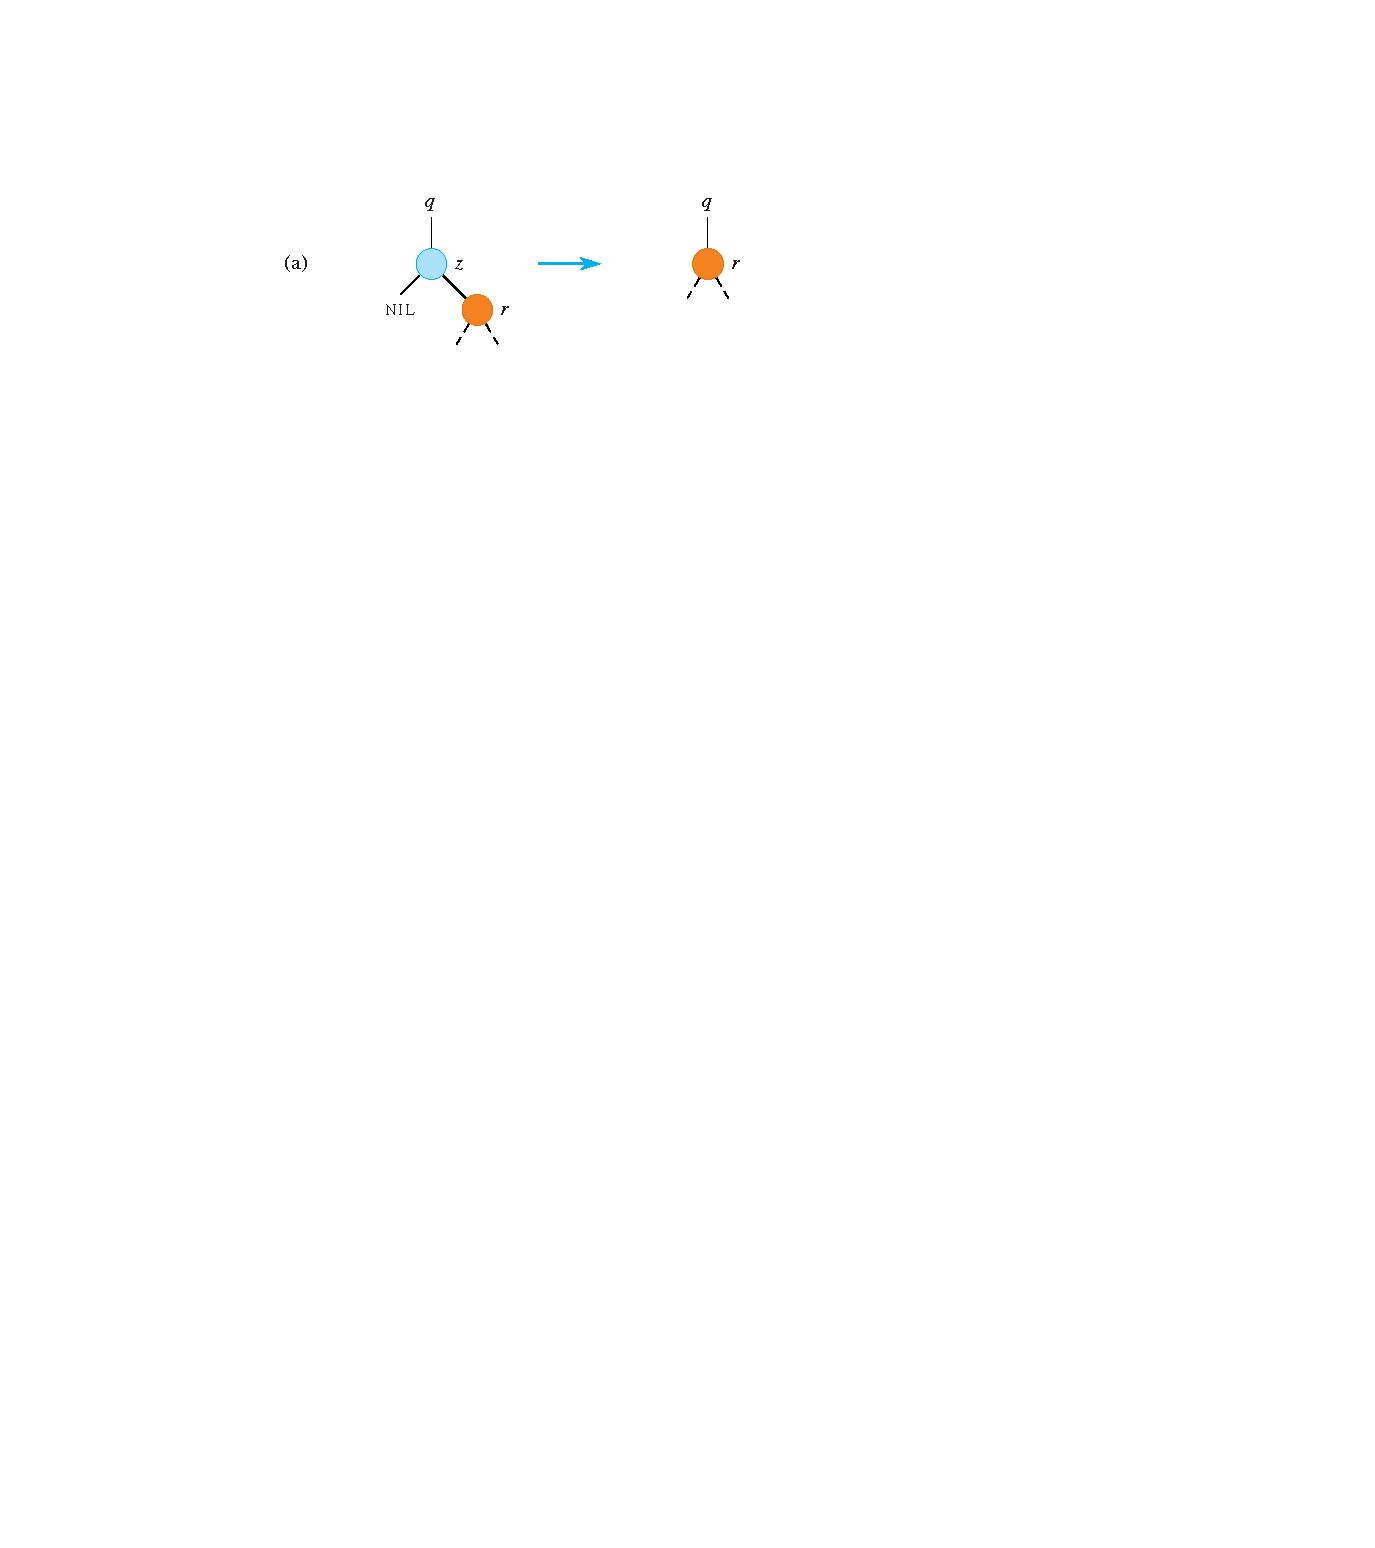
\includegraphics[width=.9\columnwidth]
				{fig/fig-CLRS12-4a}
				
			\item [b)]<2->
			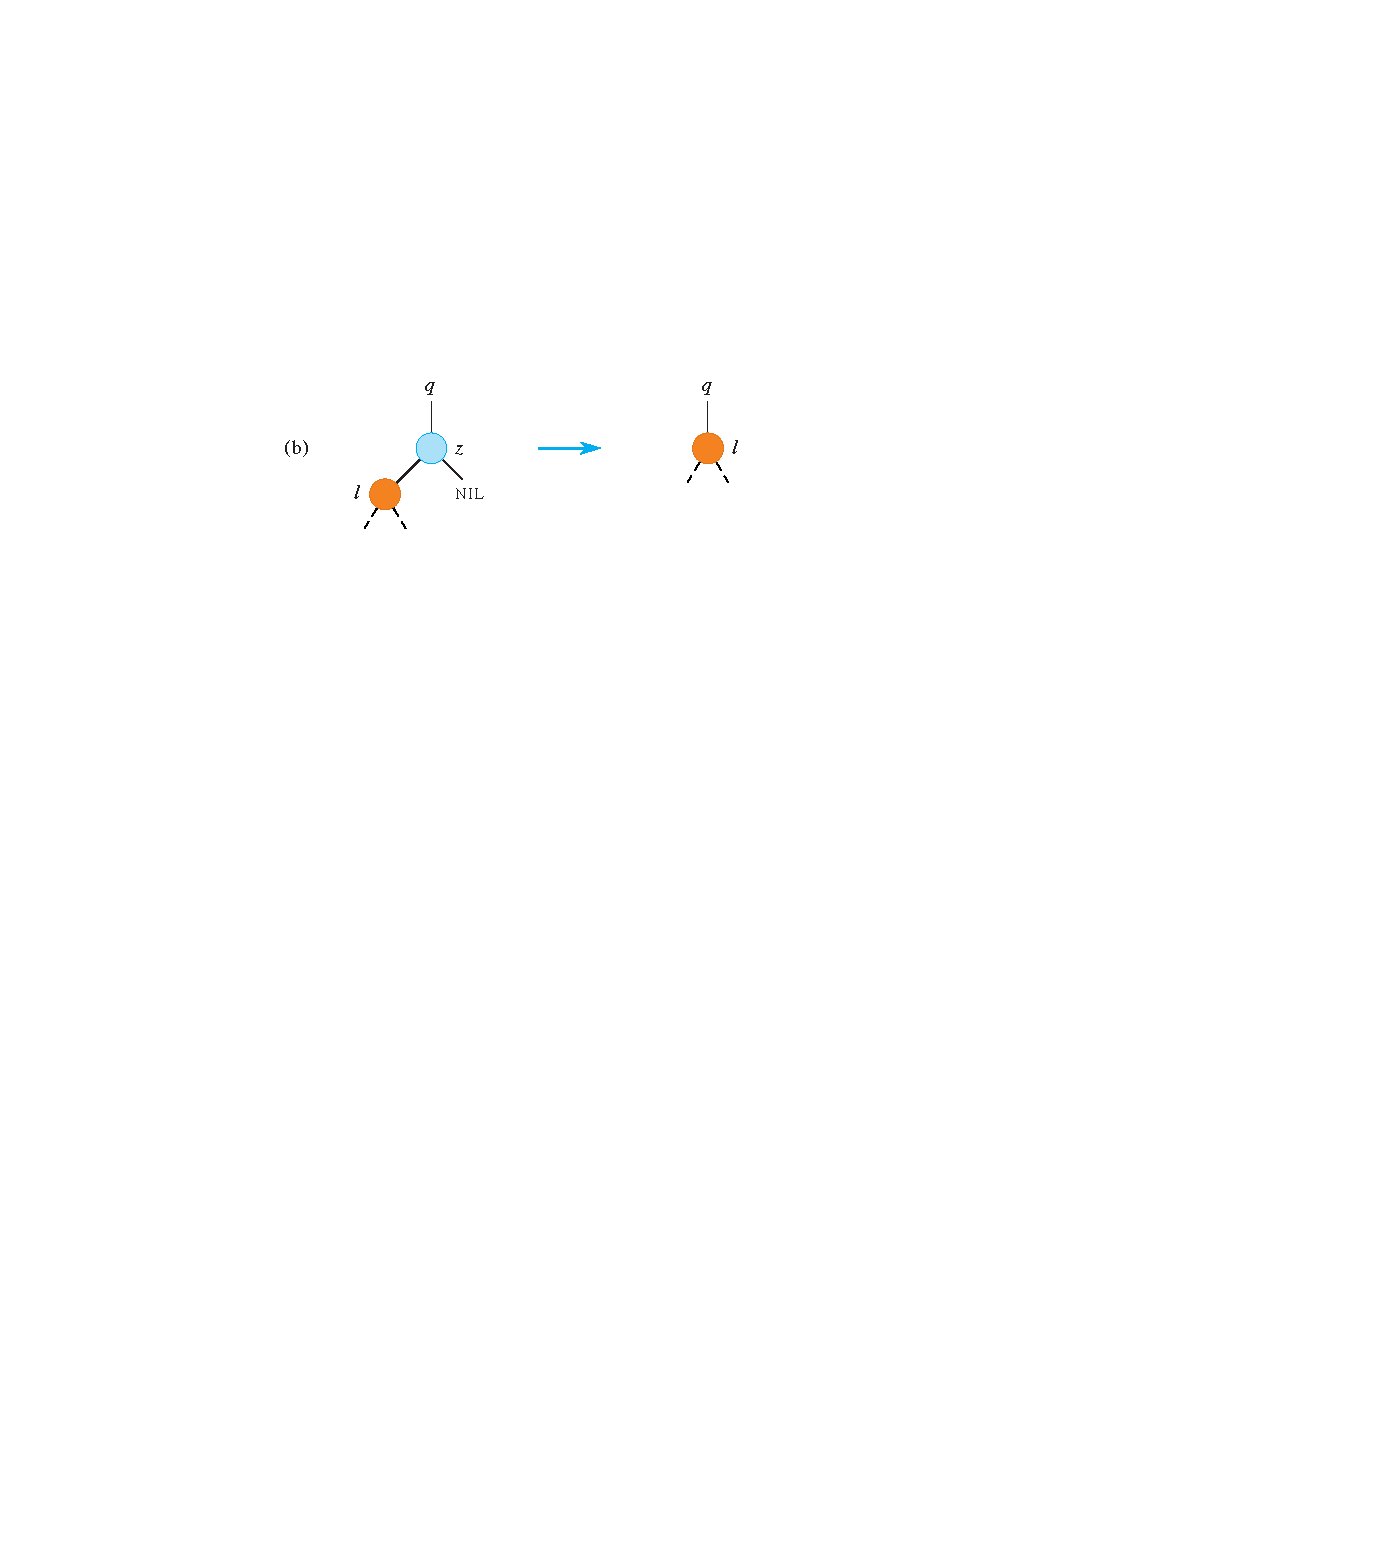
\includegraphics[width=.9\columnwidth]
				{fig/fig-CLRS12-4b}
				
			\item [c)]<3->
			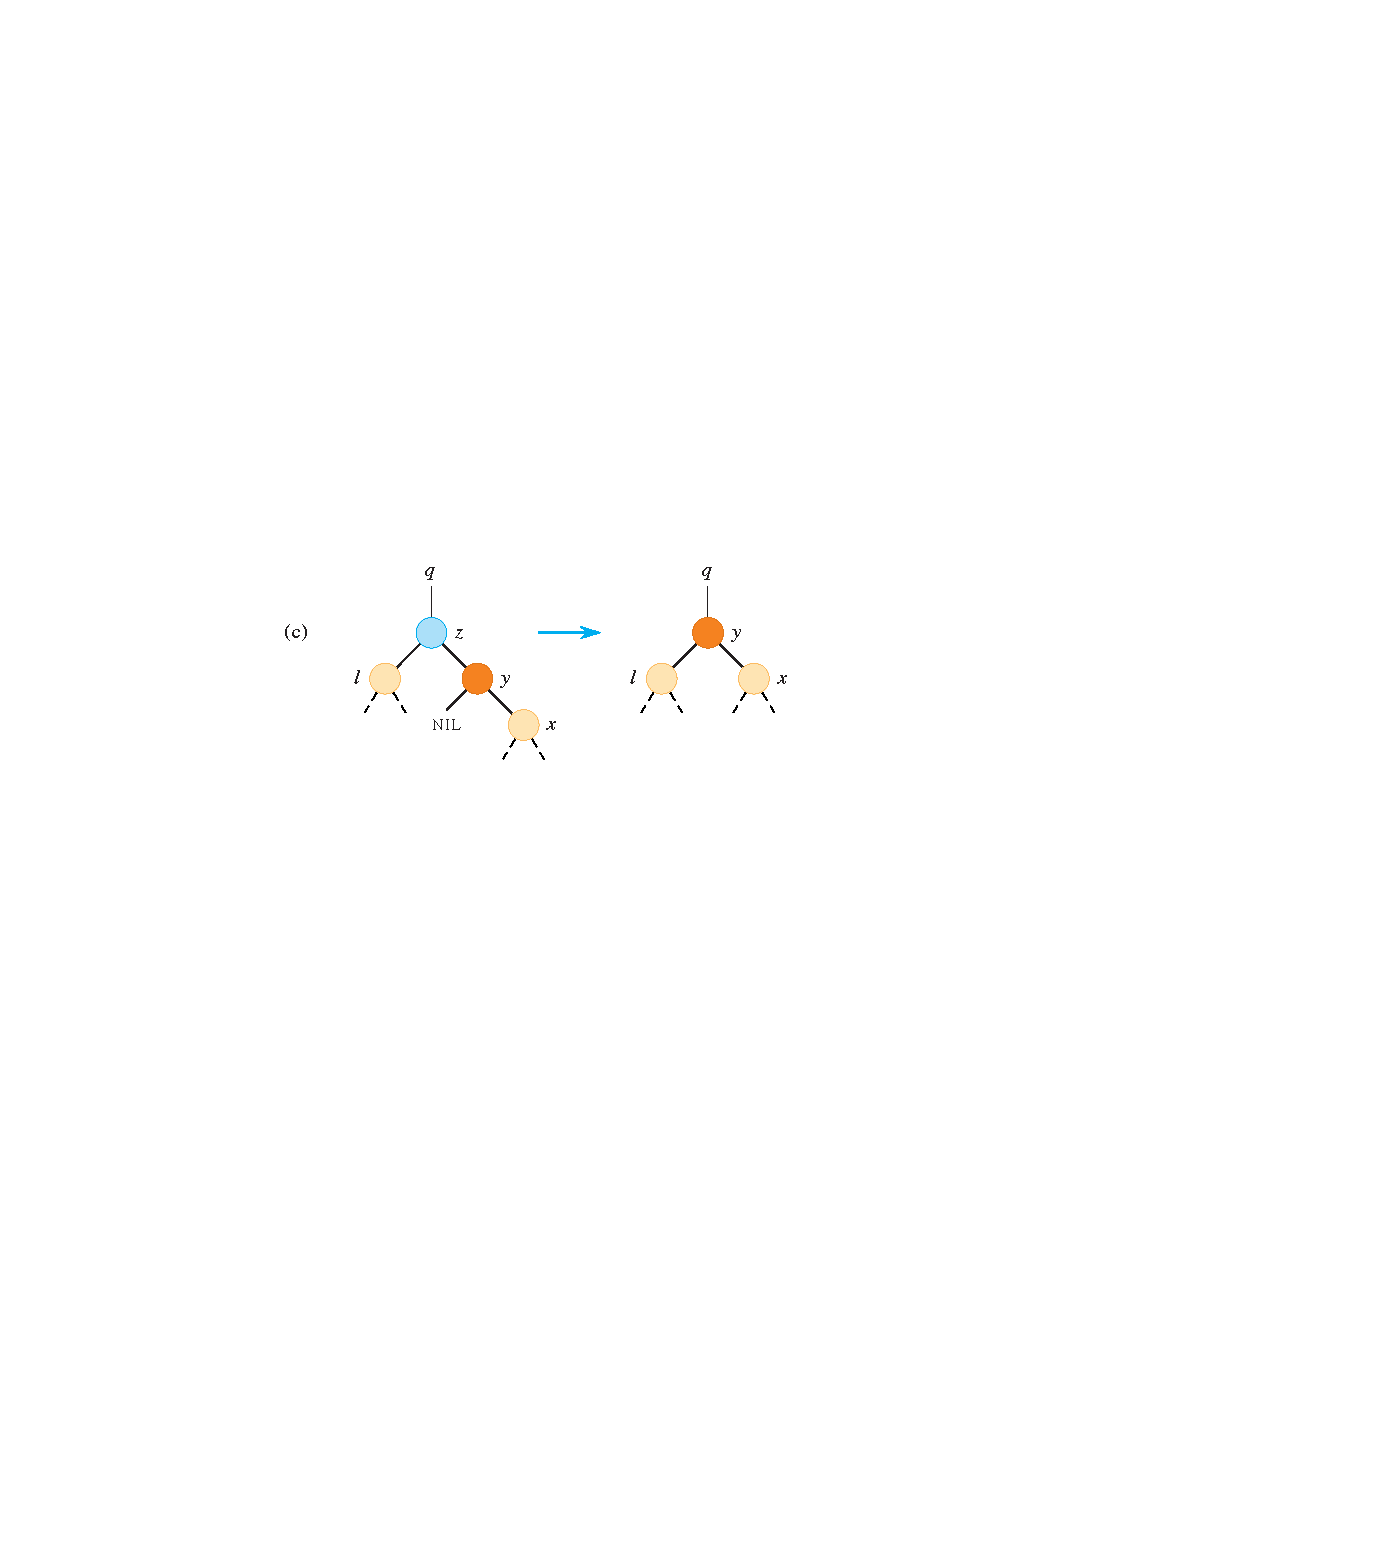
\includegraphics[width=.9\columnwidth]
				{fig/fig-CLRS12-4c}
				
			\item [d)]<4->
			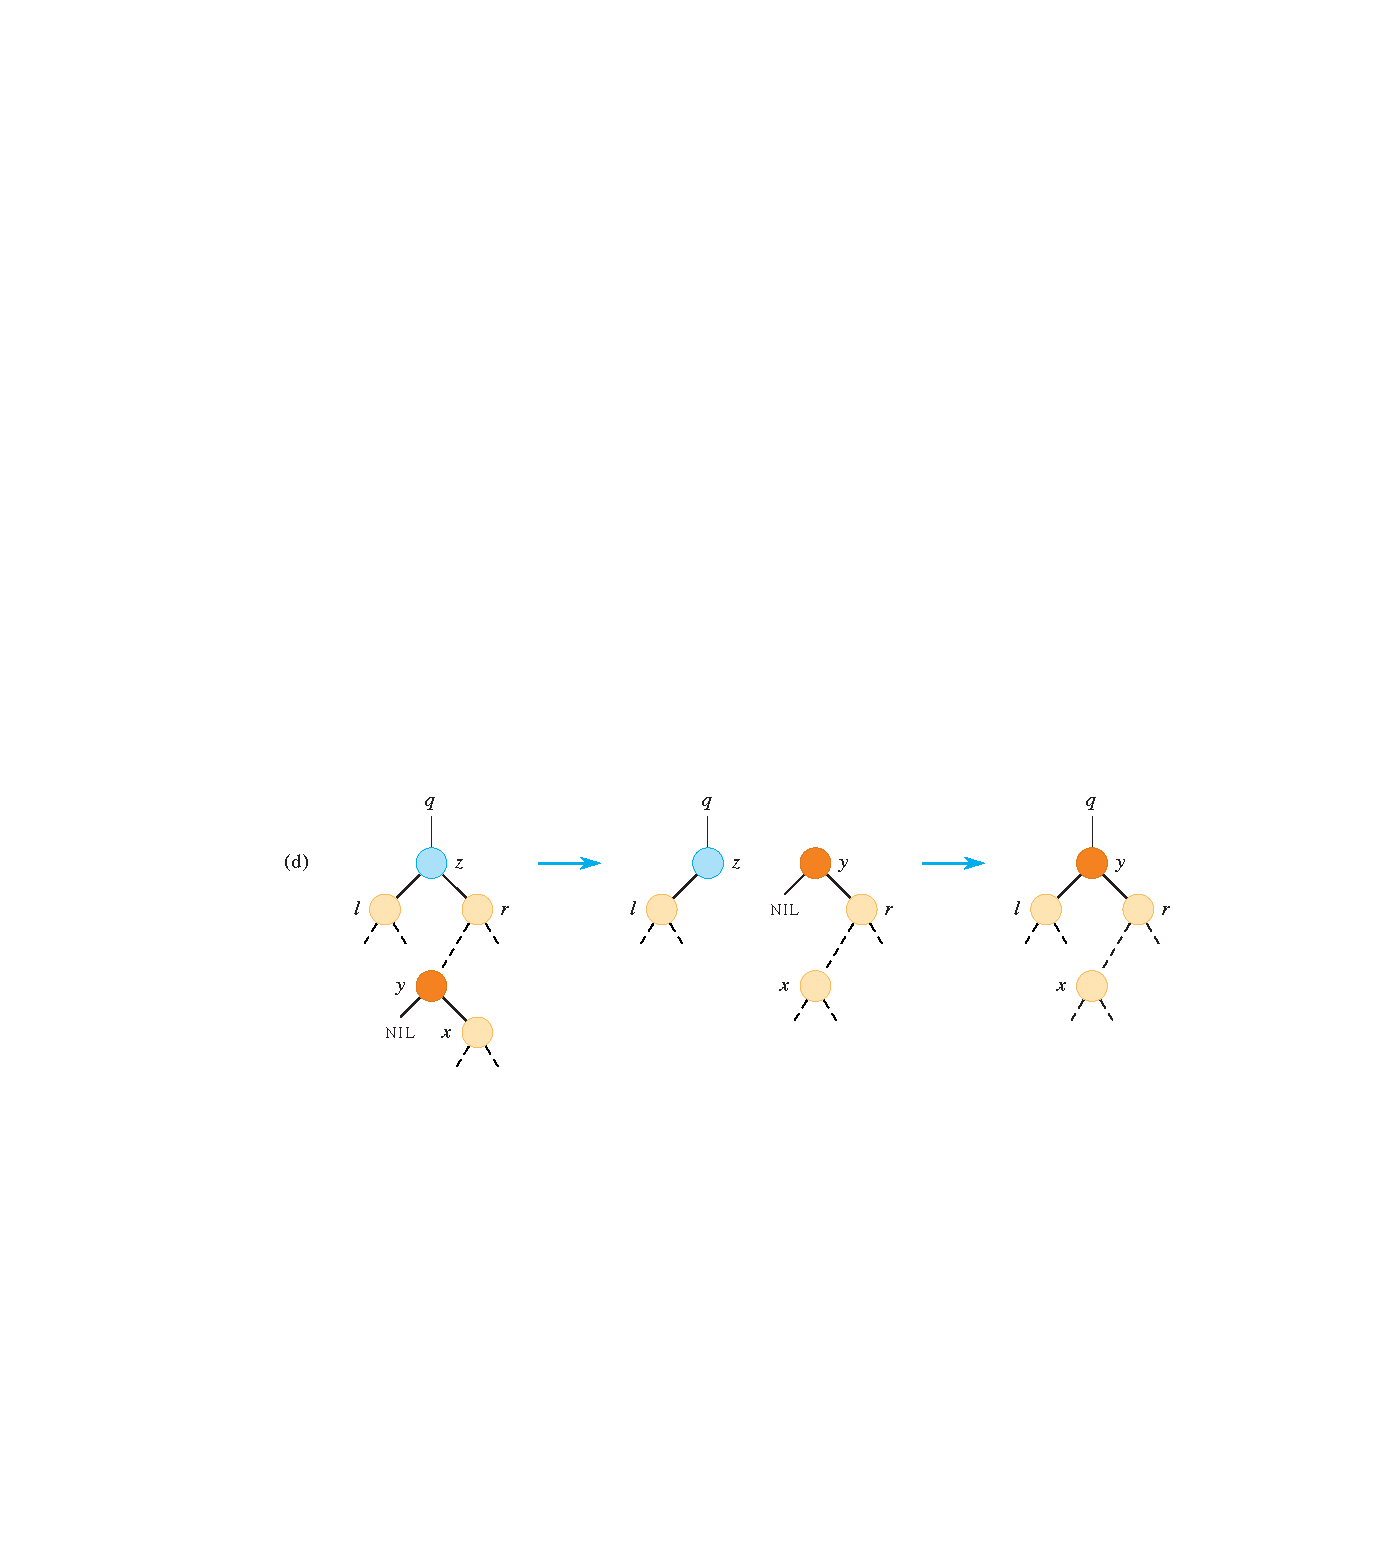
\includegraphics[width=.9\columnwidth]
				{fig/fig-CLRS12-4d}
		
		\end{itemize}
		} % fsize

	\end{column} % ++++ A
	\end{columns} % <<<<
\end{frame}
% ~~~~~~~~~~~~~~~~~~~~~~~~~~~~~~~~~~~~~~ A




% ~~~~~~~~~~~~~~~~~~~~~~~~~~~~~~~~~~~~~~ V
\begin{frame}[t]\frametitle{Transplant}
	\begin{columns}[T] % >>>>
	\begin{column}{.6\linewidth} % ++++ V
		{\scriptsize
			\begin{function}[H]
	\SetKwData{X}{\texttt{x}}
	\SetKwData{K}{\texttt{k}}
	\SetKwData{N}{\texttt{NIL}}
	%
	\SetKwData{Left}{\texttt{left}}
	\SetKwData{Right}{\texttt{right}}
	\SetKwData{Data}{\texttt{data}}
	\SetKwData{Key}{\texttt{key}}

%\tcp*[f]{{\tiny aaa}}\\
%\tcp{{\tiny aaa}}

%	\FuncSty{Transplant(}\ArgSty{T, u, v}\FuncSty{)}\\
		\If {u.p == \N}{
			T.root = v\\
		} \ElseIf {u == u.p.\Left}{
			u.p.\Left = v\\
		} \Else {
			u.p.\Right = v\\
		}
		\If {v $\neq$ \N}{
			v.p = u.p\\
		}
	\caption{Transplant(T, u, v)
		\hCite{%
			\cite{cormen2022introduction}%
		}
	}
\end{function}

		} % fsize	

		{ \scriptsize
		TRANSPLANT replaces one subtree as a child of its parent with another subtree. 
		When TRANSPLANT replaces the subtree rooted at node $u$ 
		with the subtree rooted at node $v$, 
		node $u$’s parent becomes node $v$’s parent, and $u$’s parent ends up 
		having $v$ as its appropriate child.
		} % fsize

	\end{column} % ++++ A
	\begin{column}{.4\linewidth} % ++++ V

		{\tiny 
		\begin{tikzpicture}
	\tikzset{every leaf node/.style={font=\sffamily}}
	\Tree
	[.$x$
		[.u \edge[roof]; {subtree(u)} ]
		[.$y$ ]
	]
\end{tikzpicture}
$\implies$
\begin{tikzpicture}
	\tikzset{every leaf node/.style={font=\sffamily}}
	\Tree
	[.$x$
		[.v \edge[roof]; {subtree(v)} ]
		[.$y$ ]
	]
\end{tikzpicture}
\\
\begin{tikzpicture}
	\tikzset{every leaf node/.style={font=\sffamily}}
	\Tree
	[.$x$
		[.$y$ ]
		[.u \edge[roof]; {subtree(u)} ]
	]
\end{tikzpicture}
$\implies$
\begin{tikzpicture}
	\tikzset{every leaf node/.style={font=\sffamily}}
	\Tree
	[.$x$
		[.$y$ ]
		[.v \edge[roof]; {subtree(v)} ]
	]
\end{tikzpicture}

		} % fsize

	\end{column} % ++++ A
	\end{columns} % <<<<
	
\end{frame}
% ~~~~~~~~~~~~~~~~~~~~~~~~~~~~~~~~~~~~~~ A




% ~~~~~~~~~~~~~~~~~~~~~~~~~~~~~~~~~~~~~~ V
\begin{frame}[t]\frametitle{Tree Delete}
	\begin{columns}[T] % >>>>
	\begin{column}{.7\linewidth} % ++++ V
		{\scriptsize
			\begin{function}[H]
	\SetKwData{X}{\texttt{x}}
	\SetKwData{K}{\texttt{k}}
	\SetKwData{N}{\texttt{NIL}}
	%
	\SetKwData{P}{\texttt{parent}}
	\SetKwData{L}{\texttt{left}}
	\SetKwData{R}{\texttt{right}}
	\SetKwData{Data}{\texttt{data}}
	\SetKwData{Key}{\texttt{key}}
%	\tcp*[f]{{\tiny aaa}}\\
%	\FuncSty{TreeDelete(}\ArgSty{T, z}\FuncSty{)}\\
		\If {z.\L == \N}{
			\Transplant(T, z, z.\R)\tcp*[f]{{\tiny replace z by its right child}}\\
		} \ElseIf { z.\R == \N }{
			\Transplant(T, z, z.\L)\tcp*[f]{{\tiny replace z by its left child}}\\
		} \Else {
			 y = \TreeMinimum(z.\R)\tcp*[f]{{\tiny y is z’s successor}}\\
			 \If(\tcp*[f]{\tiny is farther down the tree?}) {y $\neq$ z.\R}{	
				\Transplant(T, y, y.\R)\tcp*[f]{{\tiny replace y by its right child}}\\
				y.\R = z.\R	\tcp*[f]{{\tiny z’s right child becomes}}\\
				y.\R.\P = y\tcp*[f]{{\tiny y’s right child}}\\
			 }
			\Transplant(T, z, y)\tcp*[f]{{\tiny replace z by its successor y}}\\
			y.\L = z.\L\tcp*[f]{{\tiny and give z’s left child to y,}}\\
			y.\L.\P = y\tcp*[f]{{\tiny which had no left child}}\\
		}
	\caption{TreeDelete(T, z)
		\hCite{%
			\cite{cormen2022introduction}%
		}
	}
\end{function}


		} % fsize	

	\end{column} % ++++ A
	\begin{column}{.3\linewidth} % ++++ V

		{\small 
		\begin{tikzpicture}
	\tikzset{every leaf node/.style={font=\sffamily}}
	\Tree
	[.$12$
		[.$5$ 
			[.$2$ ]
			[.$9$ ]
		]
		[.$18$
			[.$15$ 
				[.$\textcolor{red}{13}$ ]
				[.$17$ ]
			]				
			[.$19$ ]
		]
	]
\end{tikzpicture}

		} % fsize
	
		{\footnotesize 
			\begin{tabular}{| l |}
			\hline
			Trace of {\scriptsize \TreeDelete(T, 13)}\\
			\hline
			~\\
			\hline
			\end{tabular}
		} % fsize

	\end{column} % ++++ A
	\end{columns} % <<<<
	
\end{frame}
% ~~~~~~~~~~~~~~~~~~~~~~~~~~~~~~~~~~~~~~ A



% ~~~~~~~~~~~~~~~~~~~~~~~~~~~~~~~~~~~~~~ V
\hSection{Implementation}{}{}
% ~~~~~~~~~~~~~~~~~~~~~~~~~~~~~~~~~~~~~~ A




%\subsection{NodeBST}
% ~~~~~~~~~~~~~~~~~~~~~~~~~~~~~~~~~~~~~~ V
\begin{frame}[t]\frametitle{Node for Binary Search Tree}
	\vspace{-0.3cm}
	\begin{columns}[T] % >>>>
	\begin{column}{.5\linewidth} % ++++ V
		{\tiny 
		\begin{algorithm}[H]
	\SetKwData{Data}{\texttt{data}}
	\SetKwData{P}{\texttt{parent}}
	\SetKwData{L}{\texttt{left}}
	\SetKwData{R}{\texttt{right}}
	\Begin{
		\Data\\
		\P	\tcp*[f]{{\tiny reference to the parent}}\\
		\L	\tcp*[f]{{\tiny reference to the left child}}\\
		\R	\tcp*[f]{{\tiny reference to the right child}}\\
	    
		\caption{{\footnotesize Node for Binary Search Tree}}
	}
\end{algorithm}

\hCite{%
	\cite{cormen2022introduction}%
}
		} % \tiny

		{\footnotesize
			In \hEmph{binary search tree}, 
			each node has 0, 1 or 2 subtrees.
					
			Use node with three pointers:
			\begin{itemize}
			
				\item
				\hEmph{\hCode{parent}}: points the parent
			
				\item
				\hEmph{\hCode{left}}: points the left child
			
				\item
				\hEmph{\hCode{right}}: points the right child
				
			\end{itemize}				
		} % fsize

		
	\end{column} % ++++ A
	\begin{column}{.5\linewidth} % ++++ V
		{\tiny
		\begin{center}
		\vspace{-0.5cm}
		\begin{tikzpicture}
	\tikzset{every leaf node/.style={font=\sffamily}}
	\Tree
	[.\hEmph{parent}
		[.\hEmph{node} 
			[.\hEmph{$root_{T_{L}}$}   \edge[roof]; {subtree-$T_{L}$} ]
			[.\hEmph{$root_{T_{R}}$}   \edge[roof]; {subtree-$T_{R}$} ]
		]
	]
\end{tikzpicture}		

		\end{center}
		} % fsize

		{\footnotesize			
			\hEmph{Binary Search Tree property}:
			\begin{itemize}
			
				\item
				Every node in subtree $T_{L}$ is smaller than \hCode{node}
			
				\item
				Every node in subtree $T_{R}$ is larger than \hCode{node}
						
			\end{itemize}
			
			\hQuestion{Is \hCode{node.data} smaller than  \hCode{parent.data}?}\\
			\hQuestion{Is  \hCode{node.data} larger than  \hCode{parent.data}?}\\
			
			\hRemark{Assume that data at each node is different.}
		} % fsize
	\end{column} % ++++ A
	\end{columns} % <<<<
\end{frame}
% ~~~~~~~~~~~~~~~~~~~~~~~~~~~~~~~~~~~~~~ A




% ~~~~~~~~~~~~~~~~~~~~~~~~~~~~~~~~~~~~~~ V
\begin{frame}[t]\frametitle{MyNodeBST}
	\vspace{-0.3cm}
	\begin{columns}[T] % >>>>
	\begin{column}{.5\linewidth} % ++++ V
		{\tiny 
		\begin{algorithm}[H]
	\SetKwData{Data}{\texttt{data}}
	\SetKwData{P}{\texttt{parent}}
	\SetKwData{L}{\texttt{left}}
	\SetKwData{R}{\texttt{right}}
	\Begin{
		\Data\\
		\P	\tcp*[f]{{\tiny reference to the parent}}\\
		\L	\tcp*[f]{{\tiny reference to the left child}}\\
		\R	\tcp*[f]{{\tiny reference to the right child}}\\
	    
		\caption{{\footnotesize Node for Binary Search Tree}}
	}
\end{algorithm}

\hCite{%
	\cite{cormen2022introduction}%
}
		} % \tiny

%		\vspace{.5cm}
%		{\footnotesize
		{\scriptsize 
			\hEmph{\hCode{MyNodeBST}}  implements interface \hEmph{\hCode{NodeBSTInterface}}.

		\begin{itemize}
			
			\item
			\hCode{\hEmph{T}} implements \hCode{\hEmph{Comparable}}			
			{\tiny 
			\[
			\hCode{y.data.compareTo(x.data)}
			= \begin{cases}
			      < 0, &\hCode{ y.data < x.data}, \\
			      0, &\hCode{y.data = x.data}, \\
			      > 0, &\hCode{ y.data > x.data}.
			\end{cases}
			\]
			} % \tiny			
			{\tiny 
				\lstinputlisting[style=mystyle, language=Java]
					{input/input-java-BST-compareTo.src}
			} % \tiny
			
		\end{itemize}
		
		} % fsize
	\end{column} % ++++ A
	\begin{column}{.5\linewidth} % ++++ V
		{\tiny 
			\lstinputlisting[style=mystyle, language=Java]
				{input/input-java-BST-Node.src}
		} % \tiny
		{\tiny 
			\lstinputlisting[style=mystyle, language=Java]
				{input/input-java-BST-NodeInterface.src}
		} % \tiny
	\end{column} % ++++ A
	\end{columns} % <<<<

\end{frame}
% ~~~~~~~~~~~~~~~~~~~~~~~~~~~~~~~~~~~~~~ A




%\subsection{MyBST}
% ~~~~~~~~~~~~~~~~~~~~~~~~~~~~~~~~~~~~~~ V
\begin{frame}[t]\frametitle{MyBST, constructor}
	\vspace{-0.3cm}
	\begin{columns}[T] % >>>>
	\begin{column}{.5\linewidth} % ++++ V
		{\tiny 
			\lstinputlisting[style=mystyle, language=Java]
				{input/input-java-BST-MyBST-insert.src}
		} % \tiny
	\end{column} % ++++ A
	\begin{column}{.5\linewidth} % ++++ V
		{\tiny 
			\lstinputlisting[style=mystyle, language=Java]
				{input/input-java-BST-Node.src}
		} % \tiny
		{\tiny 
			\lstinputlisting[style=mystyle, language=Java]
				{input/input-java-BST-MyBST-constructor.src}
		} % \tiny
	\end{column} % ++++ A
	\end{columns} % <<<<

\end{frame}
% ~~~~~~~~~~~~~~~~~~~~~~~~~~~~~~~~~~~~~~ A




\subsection{insert}
% ~~~~~~~~~~~~~~~~~~~~~~~~~~~~~~~~~~~~~~ V
\begin{frame}[t]\frametitle{MyBST, \hCode{insert}}
	\vspace{-0.3cm}
	\begin{columns}[T] % >>>>
	\begin{column}{.5\linewidth} % ++++ V
		{\tiny 
			\lstinputlisting[style=mystyle, language=Java]
				{input/input-java-BST-MyBST-insert.src}
		} % \tiny
	\end{column} % ++++ A
	\begin{column}{.5\linewidth} % ++++ V
		{\tiny 
			\lstinputlisting[style=mystyle, language=Java]
				{input/input-java-BST-MyBST-constructor-test.src}
			\lstinputlisting[style=mystyle, language=Java]
				{input/input-java-BST-MyBST-constructor.src}
			\hCodeOutputOnly{input/input-java-BST-MyBST-constructor-test}[2][3.7]
		} % \tiny
	\end{column} % ++++ A
	\end{columns} % <<<<

\end{frame}
% ~~~~~~~~~~~~~~~~~~~~~~~~~~~~~~~~~~~~~~ A




\subsection{search}
% ~~~~~~~~~~~~~~~~~~~~~~~~~~~~~~~~~~~~~~ V
\begin{frame}[t]\frametitle{MyBST, \hCode{search}}
	\vspace{-0.3cm}
	\begin{columns}[T] % >>>>
	\begin{column}{.5\linewidth} % ++++ V
		{\tiny 
			\lstinputlisting[style=mystyle, language=Java]
				{input/input-java-BST-MyBST-search.src}
		} % \tiny
	\end{column} % ++++ A
	\begin{column}{.5\linewidth} % ++++ V

		{\tiny 
		\begin{example}
		\begin{center}
			\begin{tikzpicture}
	\tikzset{every leaf node/.style={font=\sffamily}}
	\Tree
	[.$15$
		[.$6$
			[.$3$ 
				[.$2$ ]
				[.$4$ ]
			]
			[.$7$
				[.$~$ ]
				[.$13$ 
					[.$9$ ]
					[.$~$ ]
				]				
			]
		]
		[.$18$
			[.$17$ ]
			[.$20$ ]
		]
	]
\end{tikzpicture}

		\end{center}
		{\scriptsize 		
			\hCode{tree.search(13)} ?\\
			\hCode{tree.search(4)} ?\\				
			\hCode{tree.search(5)} ?\\				
			\hCodeOutputOnly{input/input-java-BST-MyBST-search-example}[3.5][3]
		} % fsize
		\end{example}
		} % \tiny
	\end{column} % ++++ A
	\end{columns} % <<<<

\end{frame}
% ~~~~~~~~~~~~~~~~~~~~~~~~~~~~~~~~~~~~~~ A




\subsection{minimum, maximum, successor, predecessor}
% ~~~~~~~~~~~~~~~~~~~~~~~~~~~~~~~~~~~~~~ V
\begin{frame}[t]\frametitle{MyBST, \hCode{minimum}}
	\vspace{-0.3cm}
	\begin{columns}[T] % >>>>
	\begin{column}{.5\linewidth} % ++++ V
		{\tiny 
			\lstinputlisting[style=mystyle, language=Java]
				{input/input-java-BST-MyBST-min.src}
		} % \tiny
		{\tiny 
			\lstinputlisting[style=mystyle, language=Java]
				{input/input-java-BST-LibTreBST-min.src}
		} % \tiny
	\end{column} % ++++ A
	\begin{column}{.5\linewidth} % ++++ V
		{\tiny 
		\begin{example}
		\begin{center}
			\begin{tikzpicture}
	\tikzset{every leaf node/.style={font=\sffamily}}
	\Tree
	[.$15$
		[.$6$
			[.$3$ 
				[.$2$ ]
				[.$4$ ]
			]
			[.$7$
				[.$~$ ]
				[.$13$ 
					[.$9$ ]
					[.$~$ ]
				]				
			]
		]
		[.$18$
			[.$17$ ]
			[.$20$ ]
		]
	]
\end{tikzpicture}

		\end{center}
		{\scriptsize 		
			\hCode{tree.minimum()} ?\\
			\hCode{tree.minimum(tree.root.right)} ?\\				
			\hCode{tree.minimum(tree.root.right.right)} ?\\				
			\hCodeOutputOnly{input/input-java-BST-MyBST-min-example}[3.5][3]
		} % fsize
		\end{example}
		} % fsize
	\end{column} % ++++ A
	\end{columns} % <<<<

\end{frame}
% ~~~~~~~~~~~~~~~~~~~~~~~~~~~~~~~~~~~~~~ A




% ~~~~~~~~~~~~~~~~~~~~~~~~~~~~~~~~~~~~~~ V
\begin{frame}[t]\frametitle{MyBST, \hCode{maximum}}
	\vspace{-0.3cm}
	\begin{columns}[T] % >>>>
	\begin{column}{.5\linewidth} % ++++ V
		{\tiny 
			\lstinputlisting[style=mystyle, language=Java]
				{input/input-java-BST-MyBST-max.src}
		} % \tiny
		{\tiny 
			\lstinputlisting[style=mystyle, language=Java]
				{input/input-java-BST-LibTreBST-max.src}
		} % \tiny
	\end{column} % ++++ A
	\begin{column}{.5\linewidth} % ++++ V
		{\tiny 
		\begin{example}
		\begin{center}
			\begin{tikzpicture}
	\tikzset{every leaf node/.style={font=\sffamily}}
	\Tree
	[.$15$
		[.$6$
			[.$3$ 
				[.$2$ ]
				[.$4$ ]
			]
			[.$7$
				[.$~$ ]
				[.$13$ 
					[.$9$ ]
					[.$~$ ]
				]				
			]
		]
		[.$18$
			[.$17$ ]
			[.$20$ ]
		]
	]
\end{tikzpicture}

		\end{center}
		{\scriptsize 		
			\hCode{tree.maximum()} ?\\
			\hCode{tree.maximum(tree.root.left)} ?\\				
			\hCode{tree.maximum(tree.root.left.left)} ?\\				
			\hCodeOutputOnly{input/input-java-BST-MyBST-max-example}[3.5][3]
		} % fsize
		\end{example}
		} % fsize
	\end{column} % ++++ A
	\end{columns} % <<<<

\end{frame}
% ~~~~~~~~~~~~~~~~~~~~~~~~~~~~~~~~~~~~~~ A




% ~~~~~~~~~~~~~~~~~~~~~~~~~~~~~~~~~~~~~~ V
\begin{frame}[t]\frametitle{MyBST, \hCode{successor}}
	\vspace{-0.3cm}
	\begin{columns}[T] % >>>>
	\begin{column}{.5\linewidth} % ++++ V
		{\tiny 
			\lstinputlisting[style=mystyle, language=Java]
				{input/input-java-BST-MyBST-successor.src}
		} % \tiny
		\vspace{-0.3cm}
		{\tiny 
			\lstinputlisting[style=mystyle, language=Java]
				{input/input-java-BST-LibTreBST-successor.src}
		} % \tiny
	\end{column} % ++++ A
	\begin{column}{.5\linewidth} % ++++ V
		{\tiny 
		\begin{example}
		\begin{center}
			\begin{tikzpicture}
	\tikzset{every leaf node/.style={font=\sffamily}}
	\Tree
	[.$15$
		[.$6$
			[.$3$ 
				[.$2$ ]
				[.$4$ ]
			]
			[.$7$
				[.$~$ ]
				[.$13$ 
					[.$9$ ]
					[.$~$ ]
				]				
			]
		]
		[.$18$
			[.$17$ ]
			[.$20$ ]
		]
	]
\end{tikzpicture}

		\end{center}
		{\scriptsize 		
			\hCode{tree.successor()} ?\\
			\hCode{tree.successor(tree.root.left)} ?\\				
			\hCode{tree.successor(tree.root.left.right.right)} ?\\				
			\hCodeOutputOnly{input/input-java-BST-MyBST-successor-example}[3.5][3]
		} % fsize
		\end{example}
		} % fsize
	\end{column} % ++++ A
	\end{columns} % <<<<

\end{frame}
% ~~~~~~~~~~~~~~~~~~~~~~~~~~~~~~~~~~~~~~ A




\subsection{delete}
% ~~~~~~~~~~~~~~~~~~~~~~~~~~~~~~~~~~~~~~ V
\begin{frame}[t]\frametitle{MyBST, \hCode{delete} (i)}
	\vspace{-0.3cm}
	\begin{columns}[T] % >>>>
	\begin{column}{.5\linewidth} % ++++ V
		{\tiny 
			\lstinputlisting[style=mystyle, language=Java]
				{input/input-java-BST-MyBST-delete.src}
		} % fsize
\	\end{column} % ++++ A
	\begin{column}{.5\linewidth} % ++++ V
		{\tiny 
		\begin{example}
		Node \hCode{z} has no left child.
		
		We have $ \hCode{z} < \hCode{r}.$
		\begin{center}
			\begin{tabular}{c c c}
				\adjustbox{valign=t}{			
					\begin{tikzpicture}
	\tikzset{every leaf node/.style={font=\sffamily}}
	\Tree
	[.$9(q)$
		[.$\textcolor{colorStop}{4(z)}$
			[.$.$ ]
			[.$\textcolor{colorGo}{7(r)}$ 
				[.$6$ ]
				[.$8$ ]
			]				
		]
	]
\end{tikzpicture}

				} % adjustbox
				& becomes
				&
				\adjustbox{valign=t}{	
					\begin{tikzpicture}
	\tikzset{every leaf node/.style={font=\sffamily}}
	\Tree
	[.$9(q)$
		[.$\textcolor{colorGo}{7(r)}$ 
			[.$6$ ]
			[.$8$ ]
		]				
	]
\end{tikzpicture}

				} % adjustbox
			\end{tabular}
		\end{center}
		\end{example}
		} % fsize
	\end{column} % ++++ A
	\end{columns} % <<<<

\end{frame}
% ~~~~~~~~~~~~~~~~~~~~~~~~~~~~~~~~~~~~~~ A




% ~~~~~~~~~~~~~~~~~~~~~~~~~~~~~~~~~~~~~~ V
\begin{frame}[t]\frametitle{MyBST, \hCode{delete} (ii)}
	\vspace{-0.3cm}
	\begin{columns}[T] % >>>>
	\begin{column}{.5\linewidth} % ++++ V
		{\tiny 
			\lstinputlisting[style=mystyle, language=Java]
				{input/input-java-BST-MyBST-delete.src}
		} % fsize
\	\end{column} % ++++ A
	\begin{column}{.5\linewidth} % ++++ V
		{\tiny 
		\begin{example}
		Node \hCode{z} has a left child \hCode{$\ell$}  
		but no right child.
		
		We have $ \hCode{$\ell$} < \hCode{z}.$
		\begin{center}
			\begin{tabular}{c c c}
				\adjustbox{valign=t}{			
					\begin{tikzpicture}
	\tikzset{every leaf node/.style={font=\sffamily}}
	\Tree
	[.$9(q)$ 
		[.$\textcolor{colorStop}{4(z)}$ 
			[.$\textcolor{colorGo}{2(\ell)}$  
				[.$1$ ]
				[.$3$ ]
			]				
			[.$.$ ]
		]
	]
\end{tikzpicture}

				} % adjustbox
				& becomes
				&
				\adjustbox{valign=t}{	
					\begin{tikzpicture}
	\tikzset{every leaf node/.style={font=\sffamily}}
	\Tree
	[.$9(q)$ 
		[.$\textcolor{colorGo}{2(\ell)}$  
			[.$1$ ]
			[.$3$ ]
		]				
	]
\end{tikzpicture}

				} % adjustbox
			\end{tabular}
		\end{center}
		\end{example}
		} % fsize
	\end{column} % ++++ A
	\end{columns} % <<<<

\end{frame}
% ~~~~~~~~~~~~~~~~~~~~~~~~~~~~~~~~~~~~~~ A




% ~~~~~~~~~~~~~~~~~~~~~~~~~~~~~~~~~~~~~~ V
\begin{frame}[t]\frametitle{MyBST, \hCode{delete} (iii)}
	\vspace{-0.3cm}
	\begin{columns}[T] % >>>>
	\begin{column}{.5\linewidth} % ++++ V
		{\tiny 
			\lstinputlisting[style=mystyle, language=Java]
				{input/input-java-BST-MyBST-delete.src}
		} % fsize
\	\end{column} % ++++ A
	\begin{column}{.5\linewidth} % ++++ V
		{\tiny 
		\begin{example}
		Node \hCode{z} has two children (\hCode{$\ell$} and \hCode{y}).
		Node \hCode{y} is the successor of \hCode{z}, 
		that is, \hCode{y} has no left child.
		Node \hCode{x} is the right child of  \hCode{y}.
		
		Hence,
		\hCode{y = successor(z)}  
		and $\hCode{$\ell$} <  \hCode{z} <  \hCode{y} <  \hCode{x}$.
		\begin{center}
			\begin{tabular}{c c c}
				\adjustbox{valign=t}{			
					\begin{tikzpicture}
	\tikzset{every leaf node/.style={font=\sffamily}}
	\Tree
	[.$9(q)$ 
		[.$\textcolor{colorStop}{4(z)}$ 
			[.$2(\ell)$  
				[.$1$ ]
				[.$3$ ]
			]				
			[.$\textcolor{colorGo}{5(y)}$ 
				[.$.$ ]
				[.$7(x)$ 
					[.$6$ ]
					[.$8$ ]
				]
			]				
		]
	]
\end{tikzpicture}

				} % adjustbox
				& becomes
				&
				\adjustbox{valign=t}{	
					\begin{tikzpicture}
	\tikzset{every leaf node/.style={font=\sffamily}}
	\Tree
	[.$9(q)$ 
		[.$\textcolor{colorGo}{5(y)}$ 
			[.$2(\ell)$  
				[.$1$ ]
				[.$3$ ]
			]				
			[.$7(x)$ 
				[.$6$ ]
				[.$8$ ]
			]
		]				
	]
\end{tikzpicture}

				} % adjustbox
			\end{tabular}
		\end{center}
		\end{example}
		} % fsize
	\end{column} % ++++ A
	\end{columns} % <<<<

\end{frame}
% ~~~~~~~~~~~~~~~~~~~~~~~~~~~~~~~~~~~~~~ A




% ~~~~~~~~~~~~~~~~~~~~~~~~~~~~~~~~~~~~~~ V
\begin{frame}[t]\frametitle{MyBST, \hCode{delete} (iv)}
	\vspace{-0.3cm}
	\begin{columns}[T] % >>>>
	\begin{column}{.5\linewidth} % ++++ V
		{\tiny 
			\lstinputlisting[style=mystyle, language=Java]
				{input/input-java-BST-MyBST-delete.src}
		} % fsize
	\end{column} % ++++ A
	\begin{column}{.5\linewidth} % ++++ V
		{\tiny 
		\begin{example}
		Node \hCode{z} has two children (\hCode{$\ell$} and \hCode{r})
		and its successor $\hCode{y} \neq \hCode{r}$ lies within the subtree rooted at  \hCode{r}.
		
		Hence,
		\hCode{y = successor(z)} and $\hCode{y} \neq \hCode{r}$.
		\begin{center}
			\begin{tabular}{c c c}
				\adjustbox{valign=t}{			
					\begin{tikzpicture}
	\tikzset{every leaf node/.style={font=\sffamily}}
	\Tree
	[.$11(q)$ 
		[.$\textcolor{colorStop}{4(z)}$ 
			[.$2(\ell)$  
				[.$1$ ]
				[.$3$ ]
			]				
			[.$9(r)$ 
				[.$\textcolor{colorGo}{5(y)}$ 
					[.$.$ ]
					[.$7(x)$ 
						[.$6$ ]
						[.$8$ ]
					]
				]
				[.$10$ ]
			]				
		]
	]
\end{tikzpicture}

				} % adjustbox
				& becomes
				&
				\adjustbox{valign=t}{	
					\begin{tikzpicture}
	\tikzset{every leaf node/.style={font=\sffamily}}
	\Tree
	[.$11(q)$ 
		[.$\textcolor{colorGo}{5(y)}$
			[.$2(\ell)$  
				[.$1$ ]
				[.$3$ ]
			]				
			[.$9(r)$ 
				[.$7(x)$ 
					[.$6$ ]
					[.$8$ ]
				]
				[.$10$ ]
			]
		]				
	]
\end{tikzpicture}

				} % adjustbox
			\end{tabular}
		\end{center}
		\end{example}
		} % fsize
	\end{column} % ++++ A
	\end{columns} % <<<<

\end{frame}
% ~~~~~~~~~~~~~~~~~~~~~~~~~~~~~~~~~~~~~~ A




% ~~~~~~~~~~~~~~~~~~~~~~~~~~~~~~~~~~~~~~ V
\hSection{Applications}{}{}
% ~~~~~~~~~~~~~~~~~~~~~~~~~~~~~~~~~~~~~~ A




% ~~~~~~~~~~~~~~~~~~~~~~~~~~~~~~~~~~~~~~ V
\begin{frame}[t]\frametitle{Some Applications of BST}
	\begin{columns}[T] % >>>>
	\begin{column}{.5\linewidth} % ++++ V
	    	Implement a set in math as a BST.
		\begin{itemize}

			\item
			Modify \hCode{insert} so that no duplication is allowed.

			\item
			If the BST is balanced,
			it would be fast to search, to insert and to delete in $O(\log n)$.
		\end{itemize}
	\end{column} % ++++ A
	\begin{column}{.5\linewidth} % ++++ V
	    	Database Management Systems (DBMS)
		\begin{itemize}
			\item
			DBMS keeps data in a system similar to BSTs.
		\end{itemize}
	\end{column} % ++++ A
	\end{columns} % <<<<
\end{frame}
% ~~~~~~~~~~~~~~~~~~~~~~~~~~~~~~~~~~~~~~ A




% ~~~~~~~~~~~~~~~~~~~~~~~~~~~~~~~~~~~~~~ V References bib
\begin{frame}[t,allowframebreaks]\frametitle{References}
	\setbeamertemplate{bibliography item}[text] % sets numbers in references
%	\bibliographystyle{abbrv}
%	\bibliographystyle{apalike}
%	\bibliographystyle{ieeetr}
	\bibliographystyle{IEEEtran}
	%
	\tiny\bibliography{../hbcommon/bingol-DataStructures} % bib file

	
\end{frame}
% ~~~~~~~~~~~~~~~~~~~~~~~~~~~~~~~~~~~~~~ A

% ~~~~~~~~~~~~~~~~~~~~~~~~~~~~~~~~~~~~~~~ 
\end{document}
